\newcommand{\geomQuery}[2] {
  \null %emptyline
  \textbf{\uppercase{#1}} 
  \begin{adjustwidth}{2.5em}{0pt}
    #2
  \end{adjustwidth}
}

\chapter{Background}\label{ch:background}

\section{Monte Carlo Geometry Queries}

A Monte Carlo geometry kernel must be able to robustly support the types of
geometry queries


\geomQuery{Measure}{
    Given a volume or surface in the geometry, determine properties of that entity
  such as the volume or area.
}

\geomQuery{Point Containment}{
    Given a volume and particle location, determine if the point is inside,
    outside, or on the boundary of that volume.
}

\geomQuery{Next Surface}{
  Given a volume, particle location, and particle trajectory, determine the next
  surface of the volume that the particle intersects along with the distance to
  that intersection.
}

\geomQuery{Next Volume}{
  Given a volume and surface, determine the adjacent volume on the other side of
  the surface.
}

\geomQuery{Closest Surface}{
  Given a volume and particle location, determine the distance to to the nearest
  surface of the volume in any direction.
}


\geomQuery{Surface Normal}{
  Given a surface and particle location, determine the normal vector of the
  surface at a point closest to the particle's location.
}

\section{Analytic Geometry Representations}\label{sec:analytic_geometry}

This section contains a discussion of common analytic geometry  representations
which are often used in native representations of Monte Carlo geometry.

\subsection{Implicit Surfaces}\label{subsec:implicit_surfaces}

An implicit surface is a multivariate function defined over an $ R^3 $ domain as:

\begin{equation}
    \Omega(R^3)\rightarrow R
\end{equation}

Implicit surfaces are rich and versatile representation of closed manifolds used
for modeling, simulation, and rendering. Additionally, implicit surfaces can be
used to generate triangle meshes for rasterization or rendering on GPUs
\cite{Sethian_1996} and can also be constructed from arbitrary triangle meshes
or point clouds \cite{Sigg_2006}. Implicit surfaces are defined using the
isocontour of a scalar function defined over all space unlike an
\textit{explicit} representation of a surface which defines the subset of space
which the boundary occupies. Intuitively it might seem wasteful for a definition
to be true for all space considering the relatively small amount of space the
object will occupy, however a number of powerful tools for geometric modeling
using these representations will be discussed in this section.

An isocontour of this function with the value, $v$, can be described as:

\begin{equation}
  \Omega(\vec{x}) - v  = 0 
\end{equation}

For simplicity, the boundary of an implicit surface is defined as the isocontour
for which $v=0$. As a result, inside of the surface will have a negative value
while any point outside of the surface will have a positive value.

Unlike their explicit counterparts, implicit representations allow complex
topologies of surfaces to be integrated into a single representation. This is in
part because the function is defined for all space.As a result they handle the
merging and separation of disparate volumes well. These properties allow for
straightforward representation of dynamics surfaces such as fluids though this
is not of concern in the area of radiation transport. In practice, implicit
surfaces are used to extract mesh representations of surfaces, re-sample the
model into some other proxy for the geometry, and render models via ray
tracing. Implicit surfaces are well-suited to these applications due to the
integrated geometric properties that can be quickly recovered from their
analytic forms.

Important geometric information needed for visualization and simulation can be
readily recovered from implicit surface representations. For example, a common
operation in particle transport is the determination of its containment by a
volume in the model. A quick evaluation of the implicit function for this point
will indicate its containment by the sign of the function.
%% Such a process is more complex in the case of an explicit or discretized
%% representation. Typically this involves casting a ray through the model and
%% counting up the intersections or relying on the orientation of triangle normals
%% to indicate an entering or exiting intersection. The oddness or eveness of the
%% number of crossings will then determine the points containment.
Additionally, the distance to nearest intersection with the surface from any
point in space can quickly be determined via the definition of a signed distance
function, $d(\vec{x})$, formally defined as:

\begin{align}
  & d(\vec{x}) = min(|\vec{x} - \vec{x_{I}}|) \\
  & \Omega(\vec(x))  \,s.t.  \,|\Omega(\vec{x})| = d(\vec(x)) 
\end{align}

\begin{align}
  d \, &- \, signed \, distance \, function \\
  \vec{x_{I}} \, &- \,nearest \, boundary \,intersection
\end{align}

\noindent
Meaning that implicit surface functions can be modified to meet the three
requirements of a signed distance function:

\begin{figure}[H]
  \begin{center}
    \begin{minipage}{.8\textwidth}
      \begin{itemize}
      \item $ \Omega(\vec{x}) = d(\vec{x}) = 0 $ for all $x$ on the surface boundary
      \item $ \Omega(\vec{x}) = -d(\vec{x}) $ for all $x$ inside the surface boundary
      \item $ \Omega(\vec{x}) = d(\vec{x}) $ for all $x$ outside the surface boundary
      \end{itemize}
    \end{minipage}
  \end{center}
\end{figure}

Implicit surfaces are often used in time-dependent simulations due to their
natural extension into a fourth dimension ($ \Omega(\vec{x},t) - v  = 0 $) and
thus their support for moving boundaries and changing topologies. Implicit
surfaces are often broken up and represented by groups of Boundary
REPresentations (BREP's). 

\subsection{Constructive Solid Geometry}\label{subsec:csg}

Native Monte Carlo geometries are commonly formed from a standard set of
well-behaved implicit surfaces known as general quadratics. These surfaces are
then combined through Boolean operations to form more complex objects (as shown
in Figure \ref{fig:csg_ex}).

\begin{figure}[h]
  \centering
  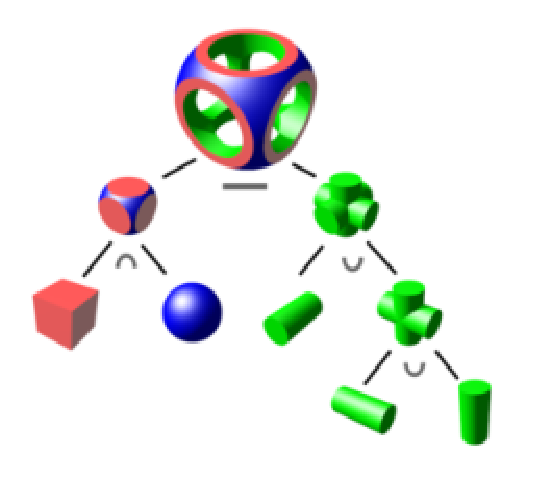
\includegraphics{csg_ex.eps}
  \caption{An example of how CSG volumes are created using boolean combinations
    of smaller objects. The union of the three orthogonal cylinders is
    subtracted from the intersection of the box and sphere on the left to form
    the final volume at the top of the figure.}
  \label{fig:csg_ex}
\end{figure}



